 \documentclass[12pt]{article}
\usepackage[a4paper, margin=.30in]{geometry}

\usepackage{array}
\usepackage{graphicx, subfig, wrapfig, fancyhdr, lastpage,makecell }
\newcommand\headerMe[2]{\noindent{}#1\hfill#2}
\usepackage[mathscr]{euscript}



\pagestyle{fancy}
\fancyhf{}

\rfoot{\em{Page \thepage \hspace{1pt} / \pageref{LastPage}}}
\begin{document}

\headerMe{Royaume du Maroc}{année scolaire \emph{2021-2022}}\\
\headerMe{Ministère de l'Éducation nationale, }{  Professeur :\emph{Zakaria Haouzan}}\\
\headerMe{du Préscolaire et des Sports}{Établissement : \emph{Lycée SKHOR qualifiant}}\\

\begin{center}

    \vspace{-1.5cm}
Devoir  N°1 \\
   Filière Tronc Commun Scientifique\\
Durée 2h00
\\
\hrulefill
\Large{Chimie 7pts - 70min}
\hrulefill\\

    %\emph{Les Trois parties sont indépendantes}
\end{center}
%end Headerss------------------------
 
    \vspace{-1.2cm}
    
\section*{Partie 1 :les espèces chimiques \dotfill (1.25pts) }
	
	1. Compléter le tableau suivant:\dotfill(0,75pts)
\begin{center}
\begin{tabular}{ | c | c | c | }
	\hline
	\textbf{Espèce chimique }& \textbf{test} & \textbf{résultat} \\\hline 
 Présence d’eau $H_2O$ & Sulfate de cuivre anhydre & ....................... \\\hline  
 acide & ............. & ........................\\\hline 
\end{tabular}
\end{center}

2. Compléter avec un ou plusieurs mots:\dotfill(0.5pt)
	\begin{itemize}
		\item Une espèce chimique présente dans la nature est une espèce chimique \dotfill
		\item Une espèce chimique fabriquée par l’homme est une espèce chimique \dotfill
	\end{itemize}
\section*{Partie 2 :L’extraction de l’eugénol du clou de girofle. \dotfill (5,75 pts) }
\hspace{0.5cm}Depuis plus d’un siècle, l’eugénol est utilisée dans la médecine pour calmer la douleur
des dents et la fièvre. 

\begin{wrapfigure}[15]{r}{0.32\textwidth}
	\vspace{-0.6cm}
	\begin{center}
    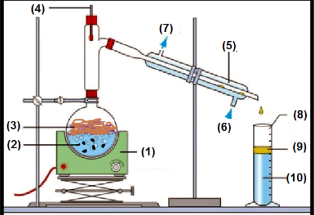
\includegraphics[width=0.32\textwidth]{./img/hydro.png}
	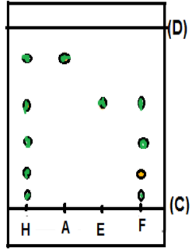
\includegraphics[width=0.2\textwidth]{./img/CCM.png}
\end{center}
\end{wrapfigure}

Dans cette partie, on s’intéresse à extraire l’eugénol du clou de
girofle, qui sont des boutons floral séché et contient une grande quantité de d’huile
essentielle trés riche en eugénol et d’acétyle eugénol.
\begin{enumerate}
	\item[I] \underline{\textbf{Première étape : l’extraction de l’eugénol.}}
		\begin{enumerate}
			\item[1.] Pour extraire l’huile essentielle des clous de girofle, on
introduit dans un ballon 100 ml d’eau distillée, 5g de clous de
girofle en poudre et quelques pierres ponce. Le ballon est placé dans
le montage suivant ci-contre.et on recueillit le distillat dans une
éprouvette graduée.
	\item[1.1.] donner le nom de ce montage, et donner son principe. \dotfill(0,5pts)
	\item [1.2.]Recopier les numéros des parties du montage et les nommer.\dotfill(1,25pts)
	\item [1.3.]Quel est le rôle de l’élément (5). \dotfill(0,25pts)
	\item [1.4.]Quel est le rôle des grains de pierre ponce\dotfill(0,25pts)

		\end{enumerate}
	\item[II] \underline{\textbf{Deuxième étape :séparation de deux phases. }}
		\begin{enumerate}
			\item [2.]On transvase le contenu de l’erlenmeyer dans une ampoule à décanter. On ajoute 10mL d’ un solvant
convenable pour la décantation. On agite le contenu de l’ampoule rigoureusement puis, on enlève le bouchon
de l’ampoule et on laisse décanter son contenu.

Le tableau ci-dessous donne quelques propriétés des solvants :
\begin{center}
\begin{tabular}{ | c | c | c | c | }
	\hline
							& Cyclohexane & dichlométhane &éthanol  \\\hline 
	Densité				    & 0,89        & 1,34          & 0,78\\\hline  
	Miscililité avec l’eau  & Non miscible& Non miscible  & miscible\\\hline  
	Solubilité de l’eugénol & Peu soluble & Très soluble & Très soluble\\\hline  
\end{tabular}
\end{center}

\item[2.1]Choisir le solvant convenable pour cette extraction. Justifier.\dotfill(0.5pts)
\item[2.2]Dessiner sur votre copie l’ampoule à décanter et donner les noms des deux phases.\dotfill(0,5pts)

		\end{enumerate}
		\vspace{0.5cm}	
	\item[II] \underline{\textbf{Troisième étape : identification de l’espèce extraite.}}

%\begin{wrapfigure}[5]{r}{0.36\textwidth}
    %\vspace{-1.8cm}
    %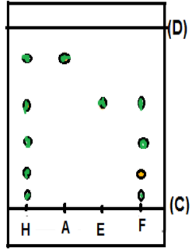
\includegraphics[width=0.36\textwidth]{./img/CCM.png}
%\end{wrapfigure}


		\begin{enumerate}
			\item[3].On réalise une chromathgraphie sur couche mince de l’huile essentielle extraite des clous de girofle. On
dépose quatre gouttes sur la plaque chromatographique.\\\textbf{(H):}L’huile essentielle extraite des clous de girofle. ; 
\\\textbf{(E):}Eugenol commercial. ; \\\textbf{(A:)}L’acétyle eugénol.
\\\textbf{(F:)}L’huile essentielle préparé à partir de feuilles de giroflier.
\\Après révélation on a obtenu le chromatogramme ci-contre.

\item[3.1.]Est-ce que l’huile essentielle (H) extraite des girofle est pure, justifier.\dotfill(0,5pts)
\item[3.2.]Que designe les deux lignes ( C ) et (D).\dotfill(0,5pts)
\item[3.3.]Quelles sont les espèces présentes dans cette huile essentielle (H) extraite des clous de girofle?\dotfill(0,5pts)

\item[3.4.]Calculer les rapports frontaux de l’eugenol commercial et de l’L’acétyle
eugénol.\dotfill(1pts) 
		\end{enumerate}
\end{enumerate}

%__________________Chimie ______________________-
%%%%%%%+_+_+_+_+_+_+_+_+_Partie1

%_____________________________________PHYSIque Partie 22222____________________________________________________________________________
\begin{center}
    %\vspace{2cm}
\hrulefill
\Large{Physique 13pts - 36min}
\hrulefill\\
    \emph{Les deux parties sont indépendantes}
\end{center}
%end Headerss------------------------

 \section*{Partie 1 :la Gravitation universelle \dotfill(10,25 pts)}

	 I. Compléter le tableau ci-dessous :\dotfill(2,25pts)
\begin{center}
\begin{tabular}{ | c | c | c | c | }
	\hline
			Distance		& Valeur en mètre(m) & Ecriture scientifique &Ordre de grandeur  \\\hline 
Diamètre d’une cellule $5\mu m$				    & \dotfill        &\dotfill &\dotfill \\\hline  
	Epaisseur d’une feuille $0,01cm$  & \dotfill& \dotfill  & \dotfill\\\hline  
	\makecell{Distance entre \\Rabat et Agadir $650 Km$} & \dotfill & \dotfill &\dotfill \\\hline  
\end{tabular}
\end{center}
 \begin{enumerate}

\item[II]. Soient deux corps ponctuels A et B de masses respectives $m_A = 10Kg$ et $m_B=20Kg$
distants de : $d =10m$.

\item Enoncer la loi de gravitation universelle\dotfill(1pts)
\item Donner les caractéristiques des deux forces de gravitation universelles               $\vec{F_{A/B}}$ et $\vec{F_{B/A}}$\dotfill(2pt)
\item Représenter sur le schéma ci-contre les  $\vec{F_{A/B}}$ et $\vec{F_{B/A}}$ en utilisant une échelle adapté.\dotfill(2pt)
\item[III.] A une altitude h de la surface de la terre, l’intensité de la pesanteur $g_0$ est donnée par la formule suivante :$g = G.\frac{M_T}{(R_T + h)^2}$.

\item En déduire l’expression de l’intensité du champ de pesanteur
$g_0$ la surface de la terre $(h=0)$ en fonction de :G,$M_T$,$R_T$.

\item Déduire la relation $g=g_0.\frac{R_T^2}{(R_T + h)^2}$.\dotfill(1.5pts)
\item Montrer que lorsque $h = 2.R_T$ On a $P=\frac{P_0}{9}$.\dotfill(1.5pts)
 \end{enumerate}



 \section*{Partie 2 :Exemples d’actions mécaniques\dotfill(2,75 pts)}

%\begin{wrapfigure}{r}{0.36\textwidth}
    %\vspace{-1.8cm}
    %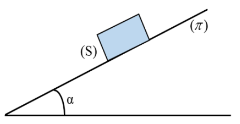
\includegraphics[width=0.36\textwidth]{./img/plan pi.png}
%\end{wrapfigure}

Un solide (S) de masse $m=100g$ est au repos sur un plan $\pi$ incliné par rapport à l’horizontale d’un angle $\alpha$ sans frottement.
\begin{enumerate}
	\item Faire le bilan des forces appliquées sur le solide (S).\dotfill(1.5pt)
	\item Représenter, sans échelle, ces forces sur le schéma ci-dessus.\dotfill(1,25pt)
\end{enumerate}











\end{document}
